\chapter{Towards Generalized Defensing Against the Dark Arts Spells}

This paper synthesizes the theoretical, practical, and specific applications of a new magical defense framework into a cohesive and universally applicable methodology. It demonstrates how a shift from reactive, spell-specific counters to a proactive, adaptable paradigm fundamentally enhances a wizard's ability to withstand the ever-evolving threats posed by the Dark Arts. This work culminates the research efforts into a singular, comprehensive blueprint for magical defense, setting a new standard for training and future research in the field.~\cite{gendart2025magic}

\section{asdf}
asdfasdf asdfasdf asdfasdf asdfasdf asdfasdf asdfasdf asdfasdf asdfasdf asdfasdf asdfasdf asdfasdf asdfasdf

\begin{table}[htbp]
\centering
\caption{Comparison of Different Defensing Techniques Against the Dark Arts}
\label{tab:defense_comparison1}
\begin{tabularx}{\textwidth}{p{2cm} X X X}
\hline
\textbf{Paper Title} & \textbf{Strengths} & \textbf{Weaknesses} & \textbf{Best Use Case} \\
\hline
Rethinking Defensing Against the Dark Arts Spells & Broad applicability, adapts to new spells & Lacks detailed spell-specific tactics & Academic/theoretical training \\
\hline
Pushing the Limits of Defensing Against the Dark Arts Spells & Finds maximum capacity of defenses, great for Aurors & High magical strain, risky for inexperienced wizards & Battle-readiness drills \\
\hline
Defensing Against the Dark Arts Spells based on Reductor Curse & Extremely powerful against physical spell constructs & Overkill for minor hexes, high collateral damage & Breaking cursed objects or barriers \\
\hline
A Survey of Defensing Against the Dark Arts Spells & Wide coverage, historical depth & Not experimental, no novel method & Reference guide for students \& teachers \\
\hline
\end{tabularx}
\end{table}



\subsection{asdf}
asdfasdf asdfasdf asdfasdf asdfasdf asdfasdf asdfasdf asdfasdf asdfasdf asdfasdf asdfasdf asdfasdf asdfasdf



\begin{figure}
    \centering
    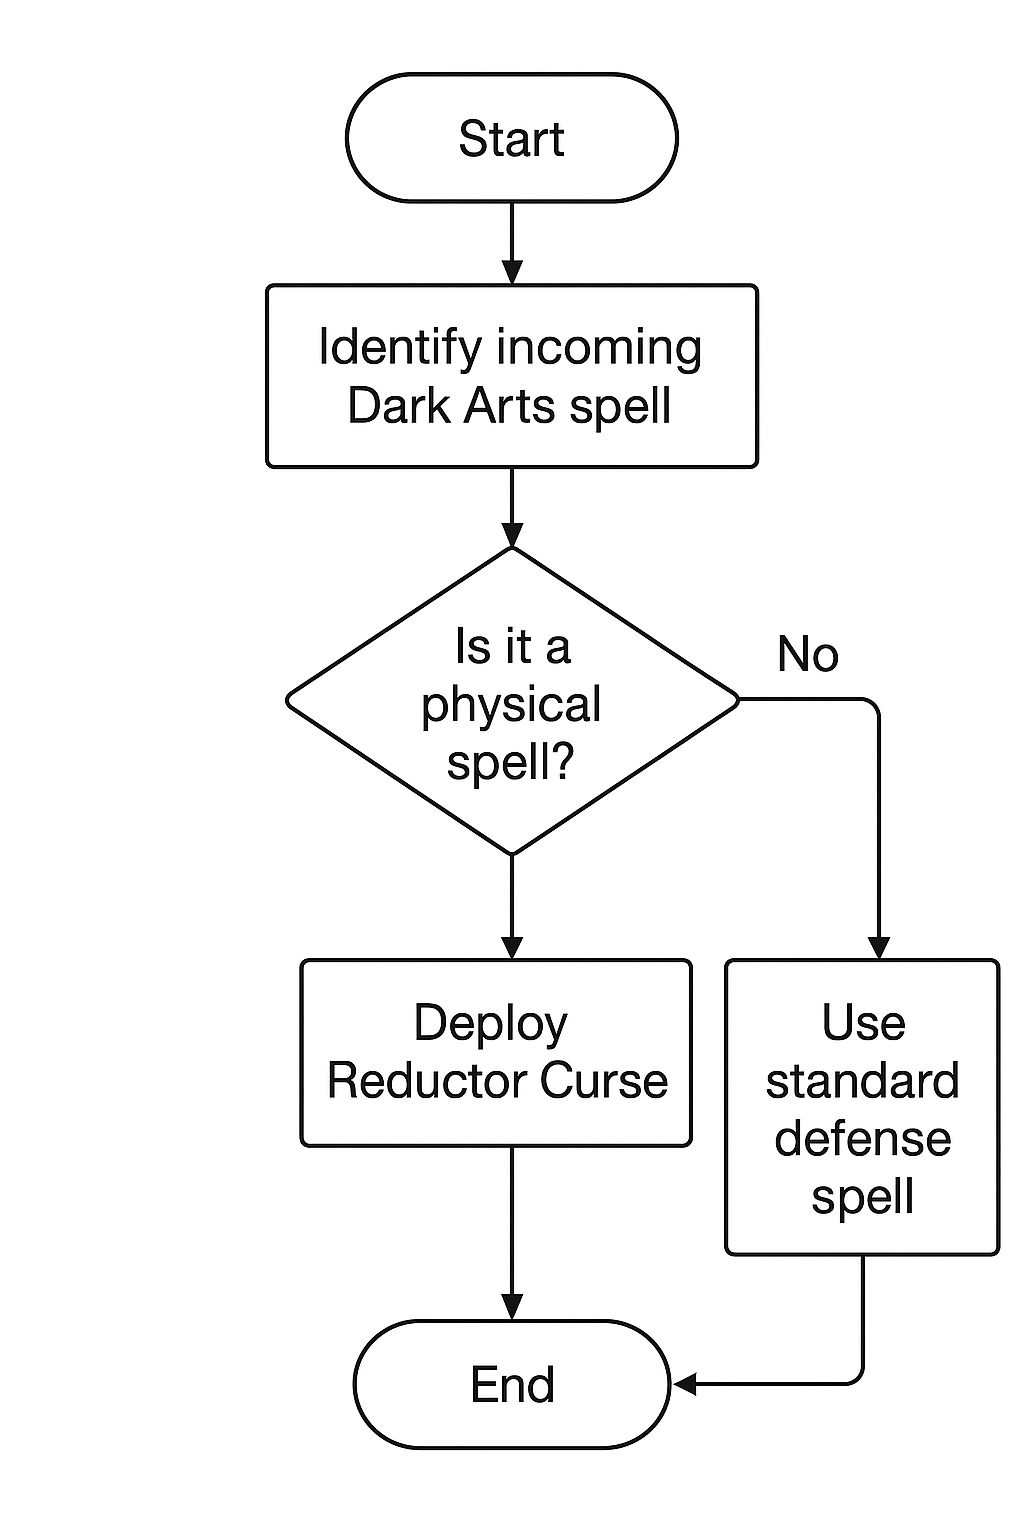
\includegraphics[width=0.5\linewidth]{images/workflow.png}
    \caption{Workflow of defensing}
    \label{fig:fig1}
\end{figure}
